%%%%%%%%%%%%%%%%%%%%%%%%%%%%%%%%%%%%%%%%%%%%%%%%%%%%%%%%%%%%%%%%%%%%%%%%%%%%%%%%
\section*{Frustration}
{   
	\usebackgroundtemplate{
		\vbox to \paperheight{\vfil\hbox to \paperwidth{\hfil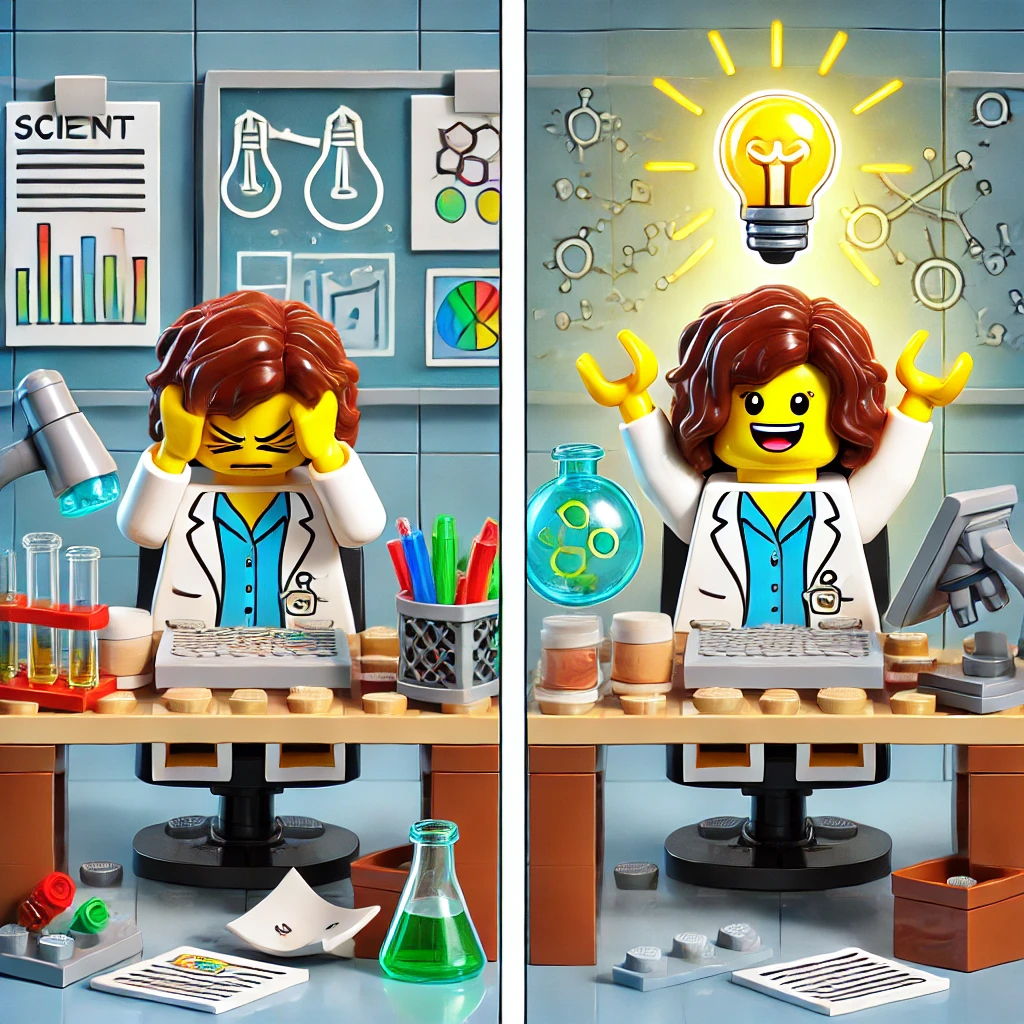
\includegraphics[height=\paperheight]{humor/DALLE_frustration_to_heureka.jpg}\hfil}\vfil}
		
	}
	\frame{
		\frametitle{Before we begin \ldots}
		\vspace{8.5em}
		\begin{mdframed}[tikzsetting={draw=white,fill=white,fill opacity=0.8,
				line width=0pt},backgroundcolor=none,leftmargin=0,
			rightmargin=50,innertopmargin=4pt,roundcorner=10pt]
			Yes, you will make mistakes. This is \ldots
			\begin{itemize}
				\item normal (it happens to \emph{all} of us)
				\item no reason to despair - you / we can learn from mistakes!
				\item just a reason to ask
			\end{itemize}
		\end{mdframed}
	    \vfill\hfil \hfill{\tiny image: own creation with DALL-E}
	}
}